\documentclass[PPFS.tex]{template/subfiles}
\begin{document}
%------------------------------------------
%	PROJECT MANAGEMENT
%------------------------------------------
\section{Project Management}
Senior Design by nature has a distributed management style, with the individual teams being self-managed for the most part. The structure which this self-management takes within the teams can vary. In team 14 it has developed into an even split with all members contributing to different parts of the project and being independently responsible for their work.

    \subsection{Team Organization}
	Team 14 consists of Daniel DeHoog, Paul Griffioen, TJ DeVries, and Ryan Siekman. The work on the project last semester was primarily doing research, and in that aspect the work was been split up primarily by the different components of the project. Daniel did the research and led the decisions concerning the displays. Paul was in charge of the sensor research. TJ worked on the server and has made the overall system diagrams for how all of these components will communicate and work together. Ryan did the research concerning the hub component. Beyond these team roles, TJ managed the schedule worksheet, Paul wrote up the submission for the Eric DeGroot Engineering fund proposal, and Ryan maintained meeting minutes and action items. All of the members of the team have been in communication with various people outside the direct team, through emails to the professors or others with whom the team has worked. These tasks have been assigned more on a basis of who the task is most relevant to, rather than having a single person do all of the email communication. Mr. Eric Walstra is the team's Industrial Mentor and Professor Michmerhuizen is the Team Advisor as well as a Course Instructor for Senior Design. Team 14's organization structure can be seen in \refFig{fig:OrganizationChart}, which includes the other Course Instructors along with a Junior Engineer, Taylor Mulder, who was part of the Business 357 team.
	
	\begin{figure}[h]
		\centering
		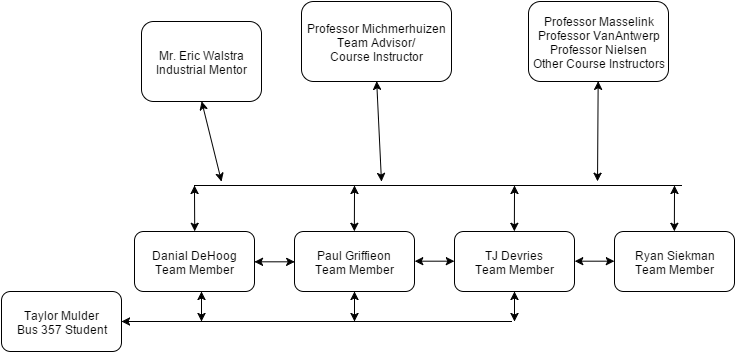
\includegraphics[width=0.75\textwidth]{OrganizationChart.png}
		\caption{Organization Chart of those Involved in the Project}
		\label{fig:OrganizationChart}
	\end{figure}
	
	The work in the spring semester of Senior Design consisted of mainly coding the software for the system to work and communicate together. The sections of the code were split up and written by a similar breakdown in components, with a different team member responsible for the software for each component. Since much of the communication needs to be coordinated, there was overlap as interpretation or encoding for the information needs to be uniform across the system. TJ wrote and worked on the server software, Dan was responsible for the hub software, Paul wrote the sensor code, and Ryan worked on the display code.

	Team meetings occurred every Monday afternoon from 3:30pm to 4:30pm after senior design class for the first semester. In the second semester more time was needed for meetings, so they moved to Tuesday mornings from 9:00am to 11:20am. Meetings were run by first covering what the previous week's action items were and discussing how they were completed or if they would continue to be an action item for the following week. Then any items that were due soon were addressed, and lastly all the future action items were assigned. This last action was usually done while discussing what the next steps of the project needed to be and the correct order and importance of them by referring to the schedule.

	Documents related to the senior design project are all kept in either GitHub or Google Drive \cite{Google Drive}. Any documents or work internal to the team is on Google Drive, while all of the documents and reports that will be turned in and all of the code written thus far for the project are kept in GitHub. The reason for keeping all of the reports and documents that will be distributed outside the team in GitHub is because these are all being written in \LaTeX. This provides more flexibility in the formatting and combining of documents written by the individuals on the team, along with version control to see what has been changed and when. The shared Google Drive folder contains the team's meeting minutes, schedule, research notes, presentation, and budget. A link to share the content of the team's Google Drive folder is in the reference section, which was cited when initially mentioned in this paragraph.
	
    \subsection{Schedule}
	Initially in trying to find a scheduling system that would work well, various options were tested, including Asana, calendar integration with Slack, Trello, and Microsoft Project. The last one, Microsoft Project, is what the initial schedule was created with. However due to its lack of online accessibility, it was exported and saved in the Google Drive folder as a spreadsheet. From there TJ continued to add functionality to it in order for the team to be able to track hours and enable better visualization of tasks and due dates. The schedule was updated with events during the team meetings or as they were assigned. Each team member edited the schedule as they spent more hours on tasks or completed them. The schedule determined what action items were assigned and what parts of the project were most critical to work on at any given time. When schedule issues arose, it was usually a matter of spending more time on tasks, delaying a due date, or deciding that one item must precede another. These issues were dealt with as they arose, and there were virtually no issues with task scheduling. However, one issue was ensuring that the schedule worked, as the functions within the spreadsheet that allow the hour tracking and views were difficult to maintain when items were added, moved around, or viewed on other sheets.
	
    \subsection{Budget}
    The budget was maintained through a spreadsheet in the team's shared Google Drive folder. It was maintained by Ryan and was updated multiple times, as the team made multiple equipment orders. It was necessary to update the budget spreadsheet as orders were made, or information on different pricing was received. The budget was not used as a management tool as it did not constrict the ability to make a prototype of the system. It only limited the size and variety of possible prototypes that could be tested.
    
    The plan is to test the system at Calvin's gym, and the budget is large enough to monitor at least two pieces of gym equipment. Any increase in the budget would allow the team to increase the scale of this testing or to test with different components than initially selected. The team obtained an increase in budget from the Eric DeGroot Engineering Fund, enabling the team to purchase more sensors than initially planned. If more machines are monitored, more data will be generated, which will help to see the accuracy and the use from an administrative side of the gym. Testing more devices would enable the team would be able to better determine what physical hardware components are more accurate or cheaper and could create a more refined final product with that knowledge. 
    
    No budget issues have arisen in the project. However, if they do then decisions will be made concerning what purchases will be more critical to the prototype than others. The primary problem which may arise being between expanding the prototype system or testing a larger variety of hardware for the system, or in the worst case, having to shrink what is currently planned for testing.  
	
	\subsection{Method of Approach}
	This project started by trying to determine a useful product, not currently available, that all members of the team would be interested in. This led to several options, most related to the Internet of Things (IoT). The problem at this point became finding a project or potential product idea that was not currently on the market, and would be feasible for the scope of senior design. Paul initially thought of an application to show users what gym equipment is in use, as gym users can get frustrated when a machine they would like to use is constantly in use. The initial idea was to accomplish this with signal analysis of the gym through a camera, using signal processing to determine where people were located and what machines they were using. Due to the large variation in gym sizes and set ups, it was determined that this would be difficult to accomplish generically for various gyms. Therefore, it was decided to implement the system using individual sensors on each machine. This approach will still have an aspect of signal analysis, though it will be done with sensor data as opposed to visual data.  
	
	With the increase in IoT technology and the growing number of sensors being used for various tasks, using sensors to determine the equipment use seemed like a more feasible idea. The next stage was what would make this more useful to the user. Being able to not just sense whether the equipment is occupied or not does not completely solve the issue of never having open equipment, as it would then just let the user know it is always occupied. Adding a reservation aspect to the system allows the user to ensure that they will have time on the desired equipment, and let other people know when it is reserved. In order to show in the gym whether equipment is reserved or not it now became necessary to add some type of display or notification ability to the equipment. It then became necessary to add a hub and server as the back end necessary to support the system.
	
	The Team has utilized Slack for communication within the team. Email is used for any communication with those outside of the team. Slack is very useful and efficient as it allows for group conversations easier than on email and still includes features like document sharing and easy access from mobile devices. 
	
\end{document}
